\chapter{Results and discussion}


This section first discusses the performance of the model, followed by
the comparison of the distributions of functional groups attributions computed 
using the different methods. Subsequently, agreement and disagreement between 
the attribution methods are examined using pairwise Spearman rank correlation. 
Next, agreement between attributions and chemical expectations is analyzed. 
Finally, the faithfulness of the attribution methods to the model is assessed 
using the fidelity metric.

 
\section{RGCN is able to accurately predict expected water solubility}


The resulting ten RGCN models, each with a different seed, have comparable results 
(\cref{fig:training_history}). 
Performance of the training data is relatively good, yielding an average $R^2$ 
of $0.9630$ and an average mean squared error (MSE) of $0.0744$ (\cref{tab:model_performance}). 
The model has a similar $R^2$ for the validation data, however, larger errors are made. 
Model performance on the test data is similar as the validation performance, showing that the 
model is able to generalize well to unseen data. Considering that most experimental data have an RMSE 
between $0.6$ and $0.7$ log(mol/L),\cite{palmer2014experimental} 
it can be concluded that the resulting model can predict water solubility of small 
molecules with decent performance.

% \begin{figure}[h]
%     \centering
%     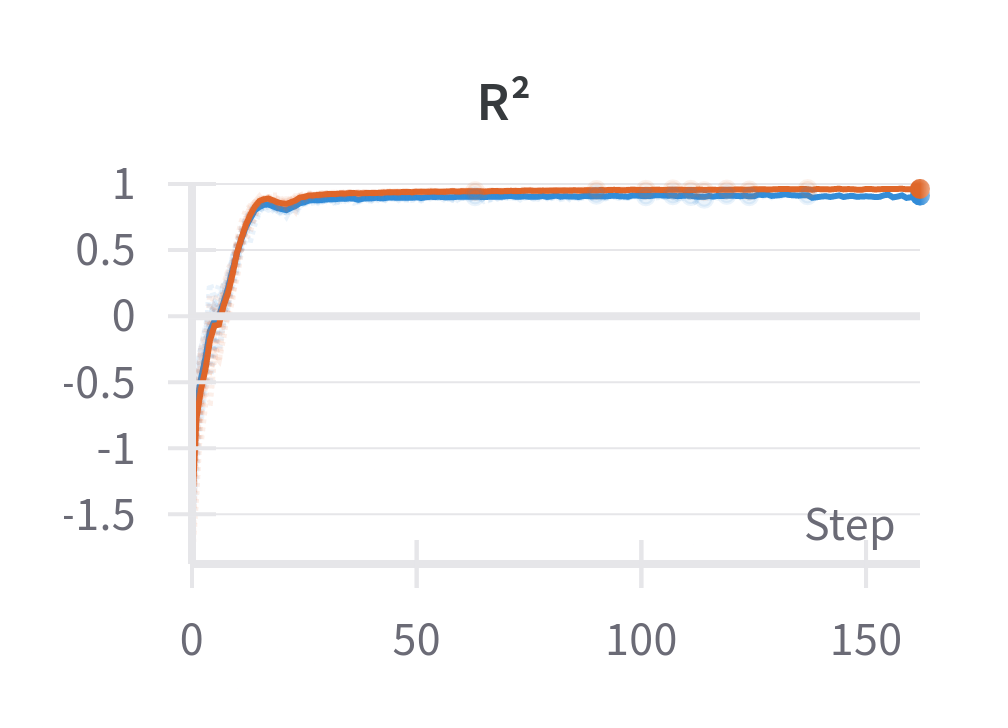
\includegraphics[scale=0.20]{rgcn_r2.png}
%     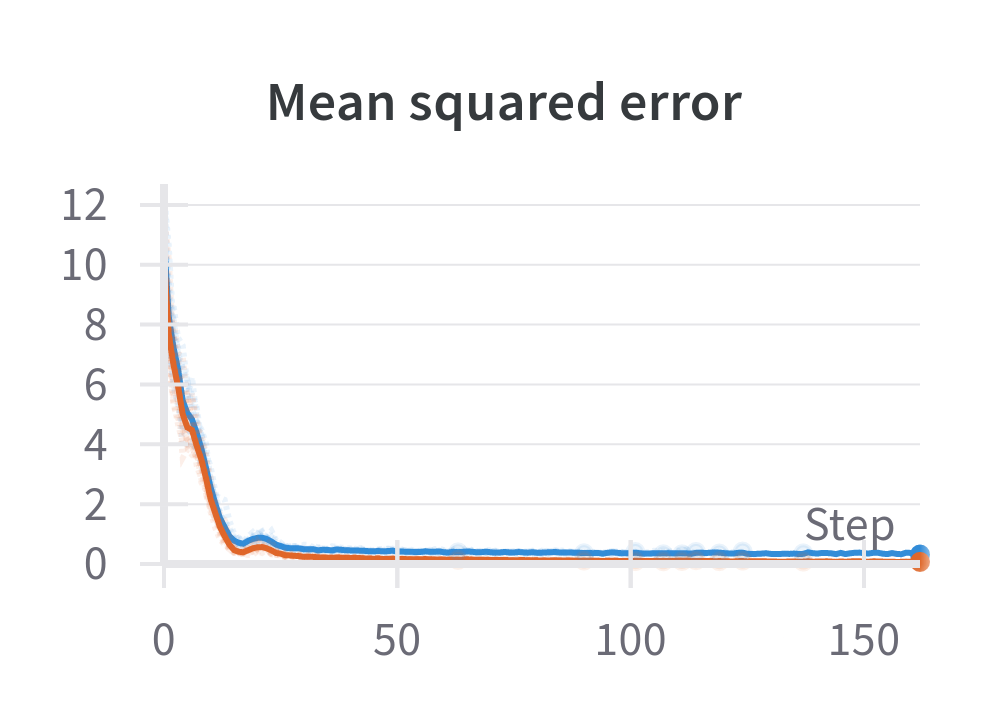
\includegraphics[scale=0.20]{rgcn_mse.png}
%     \caption{Average Mean squared error (left) and $R^2$ (right) of train (orange) and validation 
%     (blue) data during model training over the ten RGCN models, each trained using a different 
%     seed. Both metrics show a good model performance and no overfitting.}
% \end{figure}


\begin{figure}[h]
    \centering
    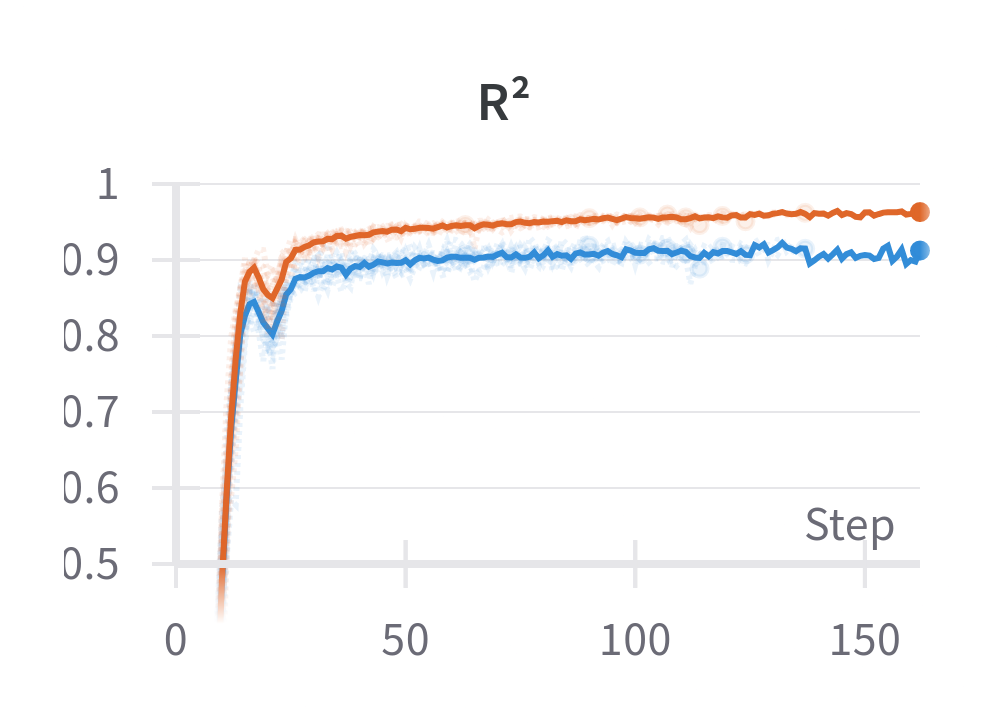
\includegraphics[scale=0.20]{rgcn_r2_zoomed.png}
    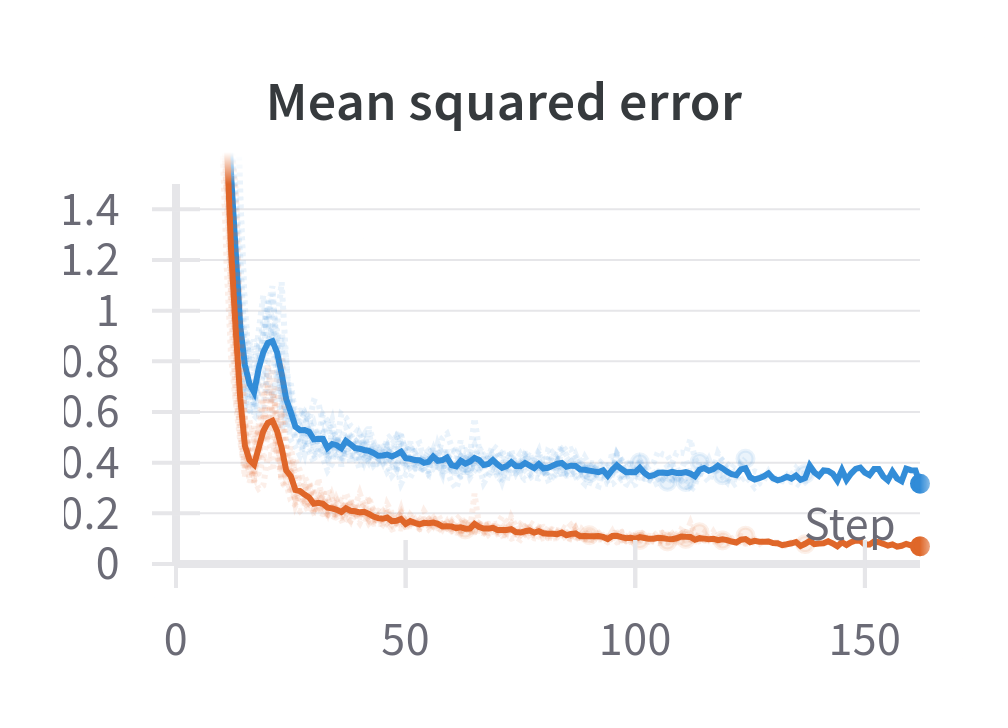
\includegraphics[scale=0.20]{rgcn_mse_zoomed.png}
    \caption{Average $R^2$ (left) and mean squared error (right) of train (orange) and validation 
    (blue) data during model training over the ten RGCN models, each trained using a different 
    seed. Both metrics show a good model performance and no overfitting. }
    \label{fig:training_history}
\end{figure}


\begin{table}[h]
    \centering
    \caption{Average $R^2$ and MSE for train, validation and test data sets with standard deviation between brackets.}
    \label{tab:model_performance}
    \begin{tabular}{ccc}
        \toprule 
       & $\pmb{R^2}$ & \textbf{MSE $\pmb{\left(\left[log(mol/L)\right]^2\right)}$} \\
        \midrule
        \textbf{Train} & $0.9630 (\pm 0.0001)$ & $0.0744 (\pm 0.0031)$ \\
        \textbf{Validation} & $0.9225 (\pm 0.0076)$ & $0.3354 (\pm 0.0120)$ \\
        \textbf{Test} & $0.9079 (\pm 0.0050)$ & $0.3193 (\pm 0.0047)$ \\
        \bottomrule 
    \end{tabular}
\end{table}



Currently, it is questionable whether the ML model effectively learns chemistry and 
if wrong predictions may be explained by chemically incorrect reasoning of the model. 
To address this, different attribution methods (SME, Shapley value and HN value) are 
compared to each other and with chemical theory. It should be noted that these attribution 
methods can reveal insights into the chemical reasoning of the model, but are not necessarily 
causal. This means that if the attributions show inconsistency with chemical theory, other 
factors could also influence the wrong prediction.


\section{Different attribution methods can result in different explanations}
\label{sec:results_different_explanations}


The attribution values sign usually shows an agreement with expectations from 
chemistry (\cref{fig:attribution_distribution_fg}). Groups that positively affect the polarity of a molecule have a 
positive attribution, while unfavorable functional groups for water solubility 
have a negative attribution. The median of HN values also shows a correct 
relationship between the functional groups. Hydroxyl groups are hydrogen bond 
acceptors and donors, so it has a superior influence on water solubility than 
a methyl ester that can only accept hydrogen bonds. Also, ethoxy has a lower 
HN value than methoxy, which is due to the larger carbon chain of ethoxy.


\begin{figure}[h]
    \centering
    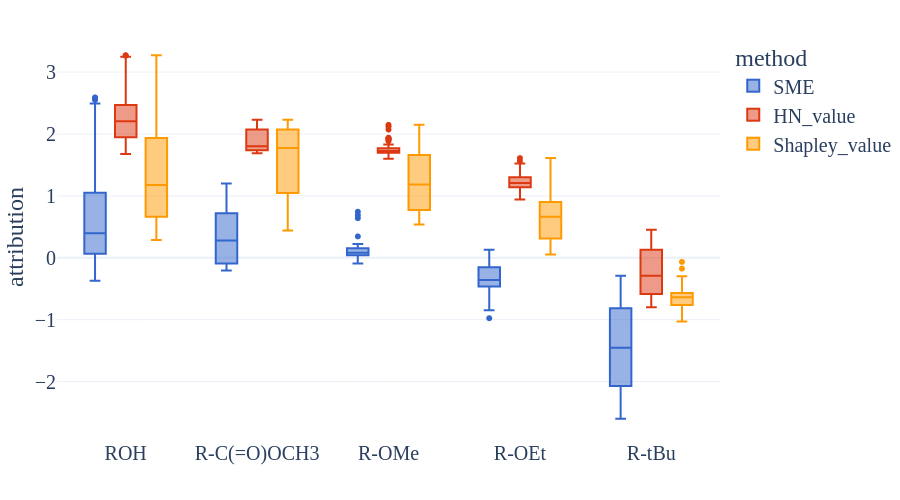
\includegraphics[scale=0.5]{attribution_distribution_functional_groups.png}
    \caption{The Shapley value, HN value, and SME attribution distributions for selected functional groups.}
    \label{fig:attribution_distribution_fg}
\end{figure}


Shapley values have mostly a broader IQR relative to the HN values. The median 
Shapley value of alcohols is lower than methyl esters, which is unexpected. 
However, SME assigns negative attributions to hydroxyl groups, which incorrectly suggests 
that hydroxyl groups can decrease the solubility of small molecules. One of those 
molecules is erythritol (\cref{fig:erythritol_explanation}), which has a predicted solubility of 0.432 log(mol/L) 
and an experimental solubility of 0.700 log(mol/L). Since the absolute prediction 
error is within acceptable limits, it would be possible that the model achieved 
this in a chemically incorrect way (i.e. clever Hans effect\cite{lapuschkin2019unmasking}). 
Clever Hans effect is a correct model prediction, however, due to the wrong reason. 
The clever Hans effect is supported by the wrong Shapley value explanation as it gives the 
apolar carbon chain a higher attribution than the hydroxyl groups. However, 
the explanation of the HN values is chemically correct, which makes it difficult 
to judge whether there is a clever Hans effect. 

Furthermore, the absolute prediction 
error for only five of the sixteen molecules with a negative SME attribution for 
hydroxyl groups is greater than the experimental error. However, those five molecules 
have a chemically consistent explanation from Shapley and HN values. The fact that only 
five of the wrong SME explanations are indeed wrongly predicted and the other attribution 
are in agreement with chemical theory tends to show that SME does not provide the correct 
model explanation. To obtain better understanding of the agreement/disagreement between 
attribution methods and the relation with absolute prediction error, a ranked based analysis is performed. 


\begin{figure}[h]
    \centering
    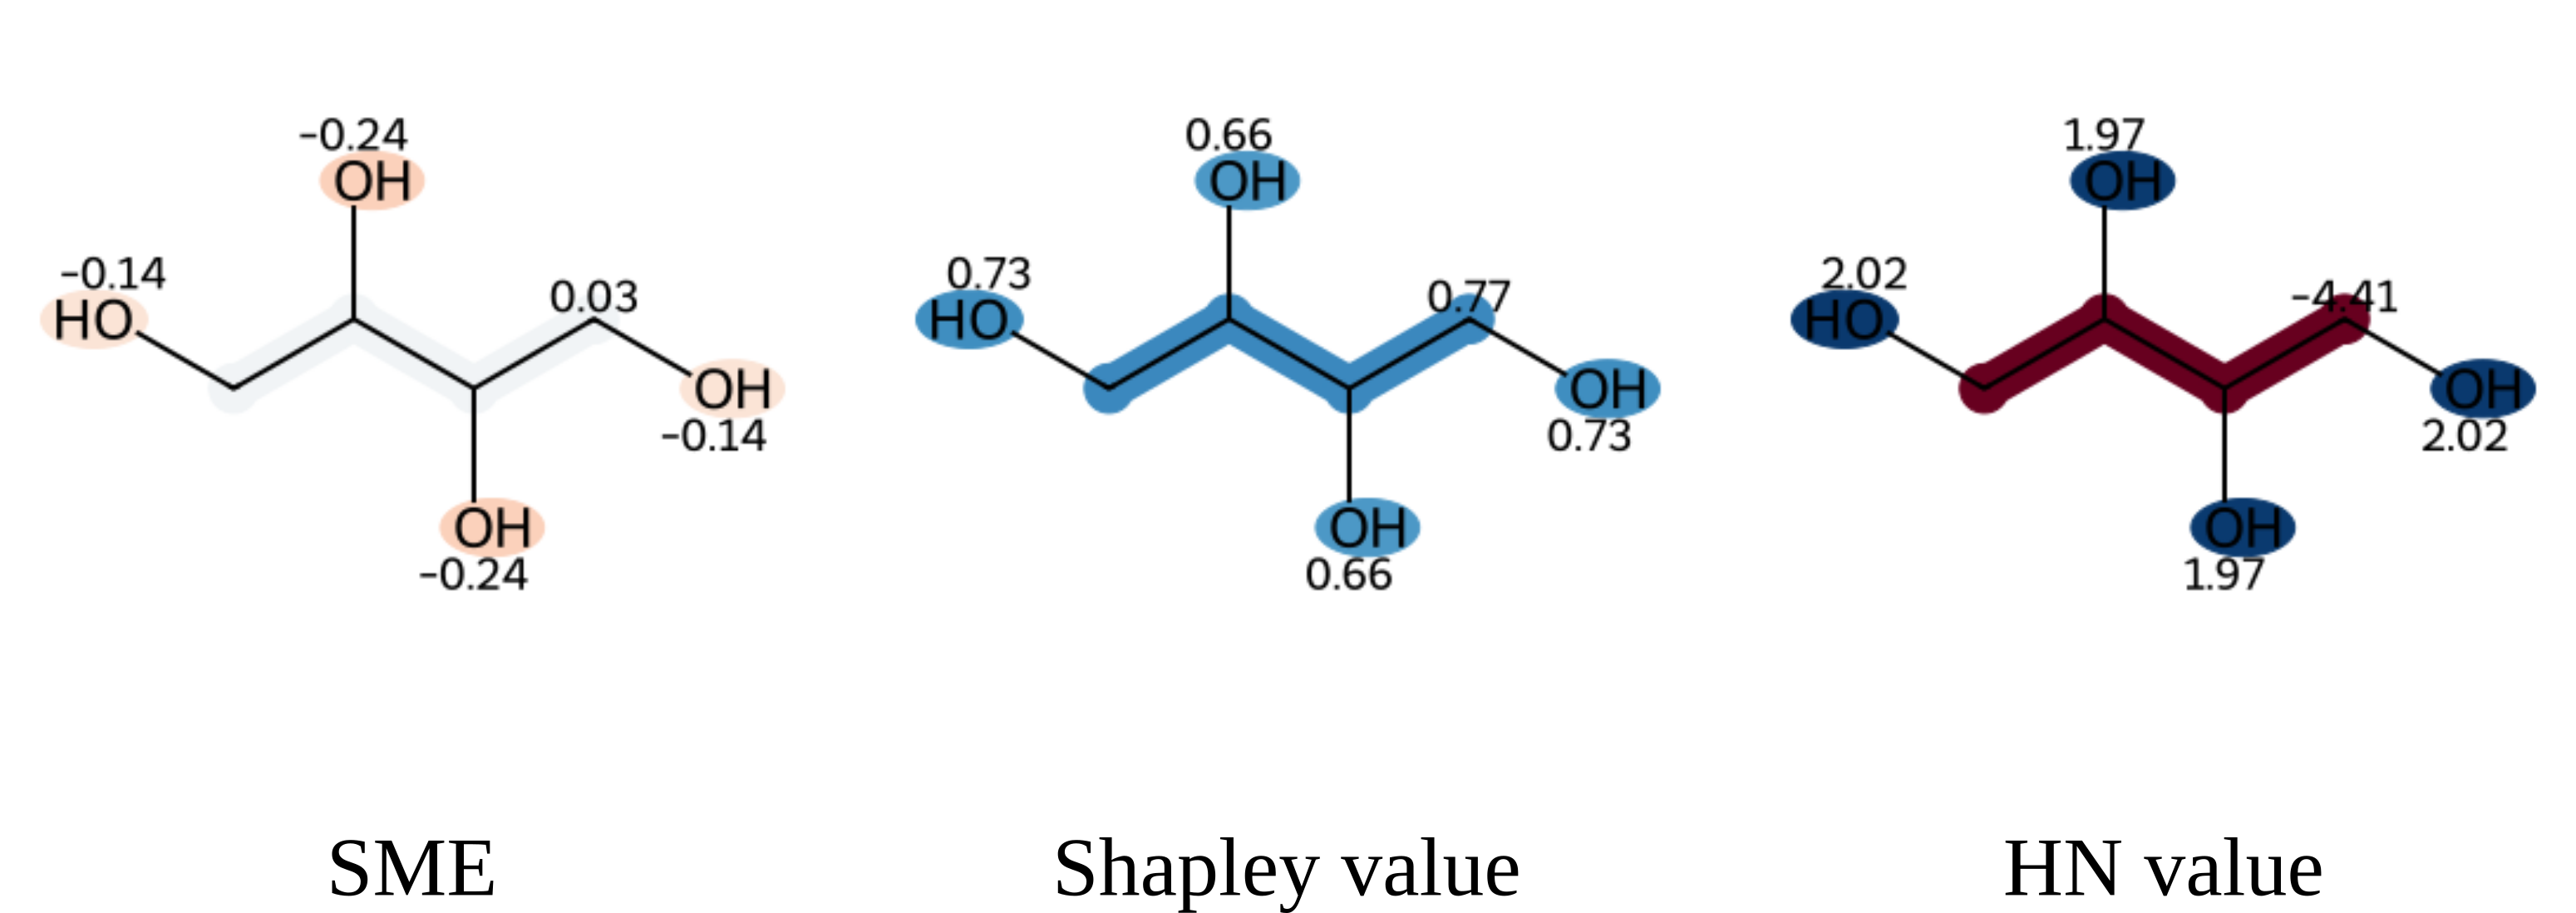
\includegraphics[scale=0.85]{erythritol_explanations.png}
    \caption{Explanations of erythritol: SME is wrong due to the negative attributions on the hydroxyl groups, 
    Shapley values are wrong since hydroxyl groups have a lower attribution than the carbon chain, HN values provide 
    a chemically correct explanation. Predicted solubility is 0.432 log(mol/L) and the experimental water solubility is 
    0.700 log(mol/L).}
    \label{fig:erythritol_explanation}
\end{figure}


\section{Absolute prediction error is not associated with the Spearman rank correlation between different attribution methods}


To get more insight into agreement or disagreement between attribution methods
and whether disagreement can be explained by the absolute prediction 
error, a ranked based approach is used. For each molecule, the substructures are ranked  
from most negative (i.e. most hydrophobic) towards most positive (i.e. most hydrophylic). 
Subsequently, the Pearson correlation is computed between the ranks of two attribution methods.


SME and Shapley value attribution rankings agree most often with each other, $78.07\%$
of the molecules have a Spearman rank correlation of one. Two molecules have 
a complete opposite explanation, where the correct ranking is provided by the 
Shapley value based ranking. Overall, no association is observed between Spearman 
correlation and the absolute prediction error. 


Perfect agreement between HN value and Shapley value ranks happens for 
$74.26\%$ of the molecules. Again at low correlation $( \le -0.5)$, the ranking based on 
the Shapley value is most often correct. Also no association between prediction error 
is observed, showing that the addition of graphical structure in the explanation 
method does not systematically change the explanation.


 

\begin{figure}[h]
    \centering
    % 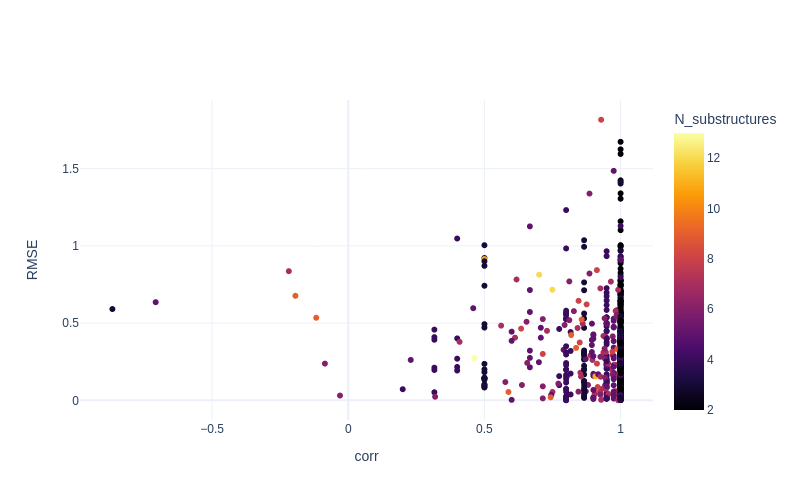
\includegraphics[scale=0.35]{../data/images/esol_rank_vs_AE_SME_Shapley_combined.png}
    % 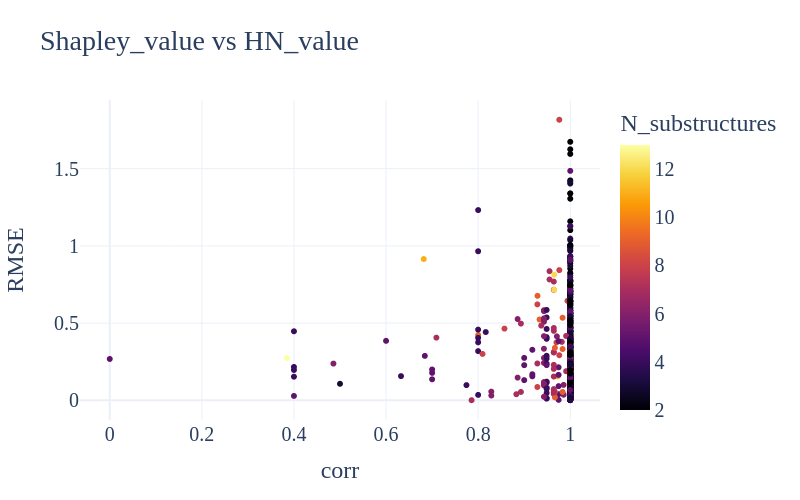
\includegraphics[scale=0.35]{../data/images/esol_rank_vs_AE_Shapley_HN_combined.png}
    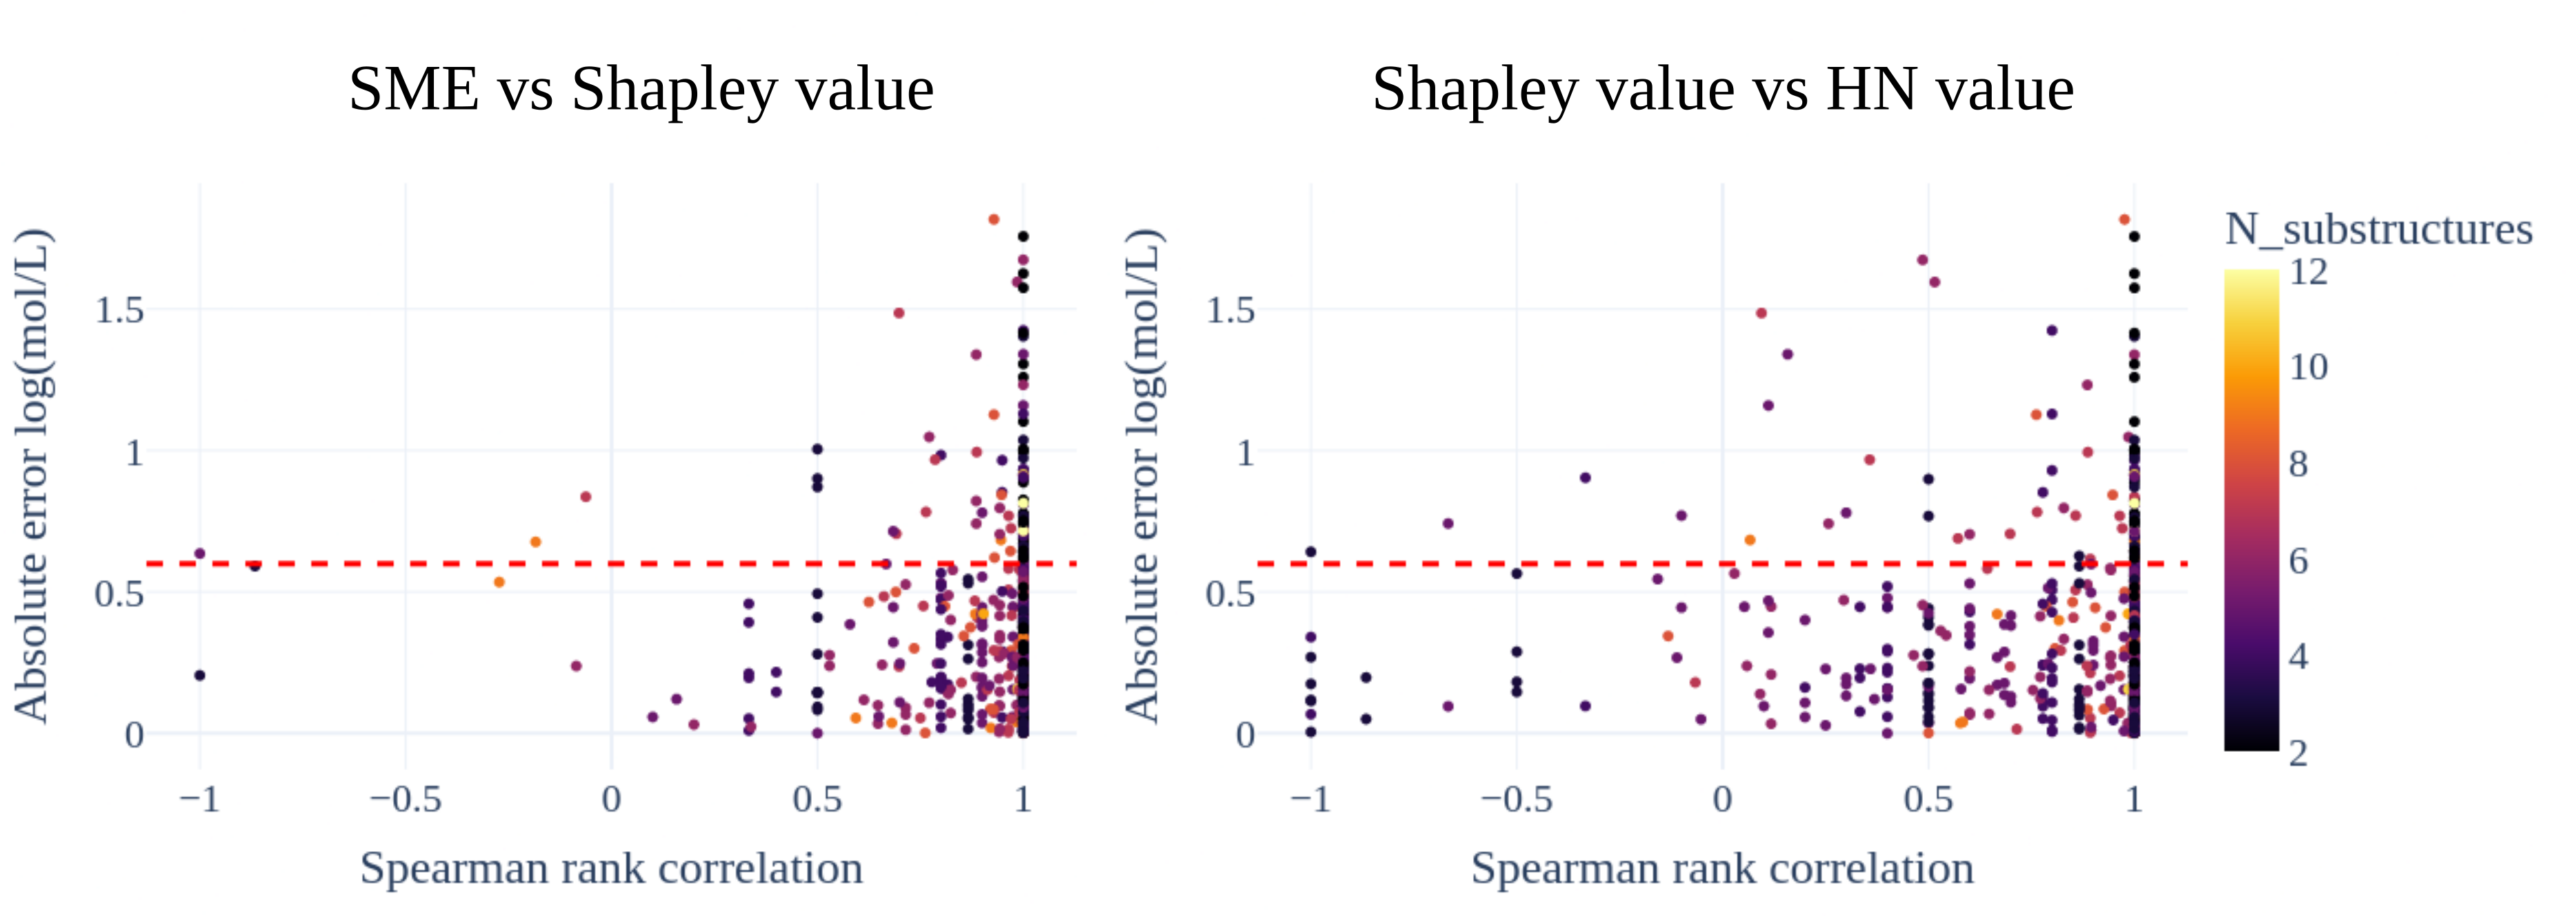
\includegraphics[scale=0.75]{rmse_vs_rank_corr_attributions.png}
    \caption{Absolute error of model prediction in function of Spearman rank correlation between 
        attributions from SME and Shapley (left) and between Shapley and HN (right) using the full 
        data set containing 1110 molecules. The red line shows experimental error of 0.6 log(mol/L).
    }
\end{figure}


\section{All attribution methods have a similar ranking with chemical expectations}

% \section{Relative evaluation of attribution methods using chemically intuitively ranked substructures shows no statistical
% significant difference between the attribution methods}


To analyze which attribution method provides the most accurate
explanation, the Spearman rank correlation is computed between the
substructures attributions and a chemically intuitive ranking of those
substructures for $100$ molecules from the test data set. Also the influence of the absolute error between model
prediction and experimental value is examined by subdividing the
molecules into two error groups based on experimental error $(<0.6 \text{ or } >=0.6)$. Since the distributions of
the Spearman rank correlations are highly skewed to the left,
non-parametric tests are used for the analysis (\cref{fig:spearman_corr_manual}). To test whether there is
a significant difference of agreement with chemical expectations between 
the different attribution methods, two Friedman tests are applied (one for each absolute error
category). Analysis of the absolute error (AE) groups for each of 
the attribution method is done using three Wilcoxon--Mann--Whitney tests.
Multiple testing is controlled by means of the Bonferonni correction, 
resulting in a significance level of $0.05/5 = 0.01$.


\begin{figure}[h]
    \centering
    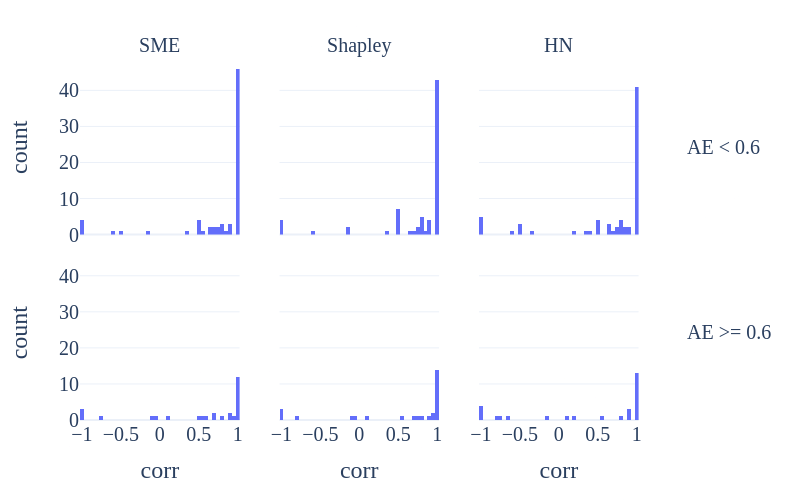
\includegraphics[scale=0.5]{spearman_rank_correlation_manual_vs_attribution.png}
    \caption{Distribution of Spearman rank correlation between an attribution method 
        and a manual ranking of substructures using chemical reasoning. The difference 
        between the two absolute error groups is mainly the intensity of high 
        correlation values.
    }
    \label{fig:spearman_corr_manual}
\end{figure}


The presence of a statistical significant difference in Spearman rank correlation
between attributions and chemically intuitive ranks for different
attribution methods is tested using a Friedman test. The null-hypothesis
assumes that there is no difference between the different attribution
methods, which would result in similar rank sums of the different
attribution methods. When the absolute prediction error is below the 
experimental error, then no statistical significant difference between 
the different attribution methods is observed (p-value $0.0154$) based 
on the Bonferonni corrected nominal level of $0.01$(\cref{fig:friedman_results}). 
Also when the absolute prediction error is above the experimental error, no significant difference 
is present between the different attribution methods (p-value $0.0148$). 
Therefore, we conclude that there is not enough
evidence in the data to reject the null hypothesis. However, considering 
that the current sample size equals $100$ and the p-values are close to the 
nominal level, it is recommended to confirm these findings in a follow up 
study with a larger sample size.


\begin{table}[h]
    \centering
    \caption{Average Spearman rank correlation between chemically ranked substructures and 
    a ranking based on attribution values.}
    \begin{tabular}{cccc}
    \toprule
    AE & SME & Shapley & HN \\
    \midrule
     < 0.6 & 0.7767 & 0.7708 & 0.6891 \\
    $\ge$ 0.6 & 0.5136 & 0.5482 & 0.3732 \\
     \bottomrule
    \end{tabular}
\end{table}


\begin{table}[h]
    \centering
    \caption{Friedman test results}
    \label{fig:friedman_results}
    \begin{tabular}{ccccc}
    \toprule
    AE & N & Statistic & df & p \\
    \midrule
     < 0.6 & 72 & 8.348 & 2 & 0.0154  \\
    $\ge$ 0.6 & 28 & 8.432 & 2 & 0.0148 \\
     \bottomrule
    \end{tabular}
\end{table}



In all attribution methods there is no significant difference between the two different
absolute error groups (p-values are $0.0214$, $0.1694$, $0.0789$ for SME, Shapley and
HN respectively). Therefore, we conclude that there is not enough evidence in the
data to reject the null hypothesis of equal distributions. 

% In other words, no attribution 
% method has a higher disagreement with chemical expectations when the prediction error 
% is above experimental error.


\section{All attribution methods are equally faithful to the ML model}


So far, different attribution methods have been compared in a more qualitative way. 
This is due to the difficulty of quantifying how correct an explanation is. The 
Spearman rank correlation between attribution and chemical expectation is one 
possible way to check the accuracy of the explanation. However, this raises the 
question whether the explanation is faithful to the model. It could be possible 
that an attribution method gives a chemically correct explanation but may not be 
representative of the model. 


Overall, all attribution methods posses a rather poor fidelity (\cref{fig:fidelity} and \cref{fig:absolute_fidelity}). 
The negative-fidelity has a median around $1.84 log[mol/L]$ for each attribution method when the absolute 
prediction error is below the experimental error. However, the distribution is rather 
broad and includes zero, meaning that sometimes removing the most negative attribution 
does not have an impact on the prediction. When the absolute prediction error is above 
the experimental error, the median negative-fidelity decreases to around $-2.40 log[mol/L]$, 
however the distribution is also more spread out. 


Similarly, the positive-fidelity is distributed around zero meaning that the removal of 
the most hydrophilic substructure does not have a significant effect on the predicted 
water solubility. A possible explanation for this is when multiple hydrophilic substructures 
are present, then it is possible that when one functional group is removed the solubility 
does only slightly decrease. 


Removing the lowest substructure with the lowest absolute attribution results in a 
smaller change of the model prediction when the attribution is closer to zero, as expected (\cref{fig:absolute_fidelity}).
However, major changes in the predicted water solubility are observed even at low absolute 
attribution values. This shows that the attribution methods are not always faithful to the model. 


\begin{figure}[h]
    \centering
    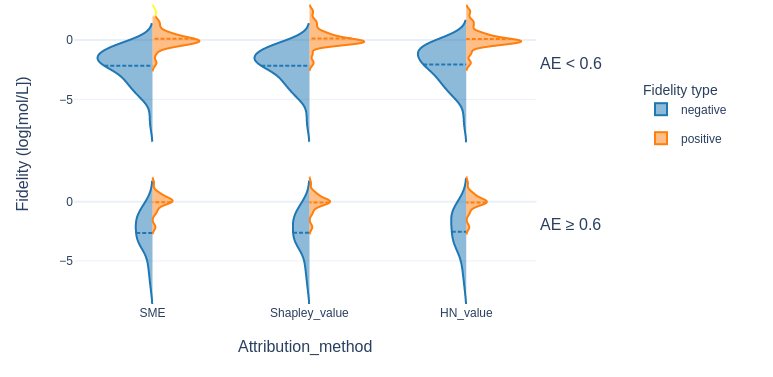
\includegraphics[scale=0.5]{fidelity_2.png}
    \caption{Distribution of fidelity obtained by removing the most positive 
        attribution (right side) or the most negative attribution (left side).
        Fidelity is computed for 100 molecules from the test data set.
    }
    \label{fig:fidelity}
\end{figure}


\begin{figure}[h]
    \centering
    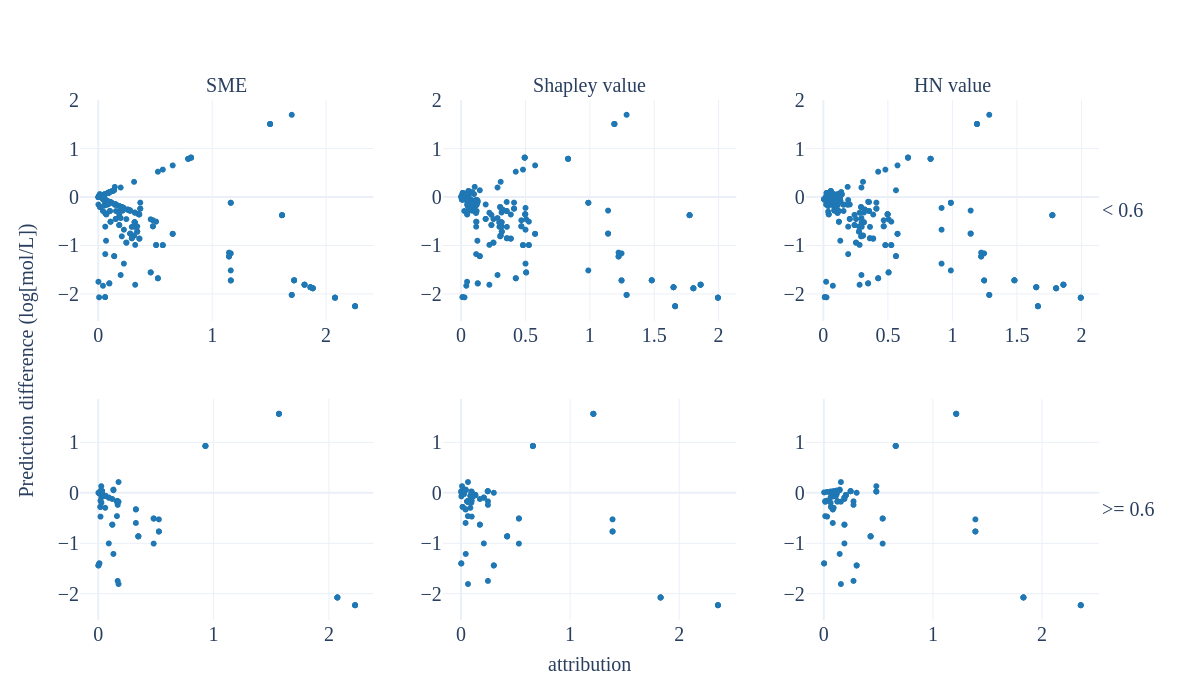
\includegraphics[scale=0.35]{absolute_fidelity_3}
    \caption{Fidelity obtained by removing the substructure 
        with the lowest absolute attribution in function of the smallest absolute attribution value.
        Fidelity is computed for 100 molecules from the test data set.
    }
    \label{fig:absolute_fidelity}
\end{figure}
